%Factor Graph Tutorial
%HU, Pili
%Update: 20120330

%HU, Pili
%Create: 20120330
%Modify: 20120330
%The unified entry to include in my tutorial series

%HU, Pili
%Create: 20110910
%Modify: 20120330
%purpose of this file is to gather commonly used
%mathematical abbreviations, to speed up writing
%notes

\documentclass[11pt,a4paper]{article}
\usepackage[utf8x]{inputenc}
\usepackage{ucs}
\usepackage{amsmath}
\usepackage{amsfonts}
\usepackage{amssymb}
\usepackage{amsthm}
\usepackage{url}
\usepackage{graphicx}

\usepackage{fancyhdr}
\pagestyle{fancy}
\fancyhead{}

%=====Calculus======
%the following commands are not originated by me
%I pick them from http://www-solar.mcs.st-and.ac.uk/~clare/Latex/
%the following line controls the style of patial derivative
%1), use \dfrac, height is larger, looks good. 
%2), use \frac, also work, but space looks limited. 
\newcommand{\myfrac}[2]{\dfrac{#1}{#2}}
\newcommand{\diff}[2]{\myfrac{{\rm d}#1}{{\rm d}#2}}
\newcommand{\ndiff}[3]{\myfrac{{\rm d}^{#3}#1}{{\rm d}#2^{#3}}}
\newcommand{\pdiff}[2]{\myfrac{\partial #1}{\partial #2}}
\newcommand{\npdiff}[3]{\myfrac{\partial^{#3} #1}{\partial #2^{#3}}}
\newcommand{\e}[1]{\ensuremath{{\rm e}^{#1}}}
\newcommand{\ldiff}[2]{\ensuremath{{\rm d}#1/{\rm d}#2}}
\newcommand{\lpdiff}[2]{\ensuremath{\partial#1/\partial#2}}
\newcommand{\lnpdiff}[3]{\ensuremath{\partial^{#3}#1/\partial#2^{#3}}}
\newcommand{\dif}[1]{\mathrm{d}#1}

%20120330
%The reason I don't copy the original file as a whole
%is that it contains too many individually preferred 
%definitions. 
%
%I start with those basic symbols and adapt them in use. 

%=====Matrix======
\newcommand{\tr}[1]{\mathrm{Tr}\left[#1\right]}
\newcommand{\tran}[1]{#1^\mathrm{T}}
%The following shorthand of matrix may be convenient. 
%However, it is so short that I'm worried it may 
%collide with something else. I don't use at present.
%\newcommand{\m}[1]{\mathbf{#1}}
\newcommand{\adj}[0]{\mathrm{adj}}

%=====Theorem definitions=====
\newcounter{mytheoremorder}
\newtheorem{mydef}{Definition}
\newtheorem{myaxm}{Axiom}
\newtheorem{mythm}[mytheoremorder]{Theorem}
\newtheorem{myprop}[mytheoremorder]{Proposition}
\newtheorem{myex}{Example}

%=====Optimization====
\DeclareMathOperator*{\argmax}{arg\,max}
\DeclareMathOperator*{\argmin}{arg\,min}
\newcommand{\maximize}[0]{\mathrm{Maximize~}}
\newcommand{\minimize}[0]{\mathrm{Minimize~}}

%=====Probability====
\newcommand{\E}[0]{\mathbb{E}}
\newcommand{\var}[0]{\mathrm{Var}}
\newcommand{\cov}[0]{\mathrm{Cov}}

%=====Quick and Unified Reference====
%20120505
%Usage: \eq{\ref{xxx}}
%The reason I keep "\ref" away from definition, 
%and let user type it every time is that: 
%currently I'm working on Texmaker, and it can 
%trigger a selection panel when the sequence 
%"\ref" is found. Maybe further configuration of 
%texmake can make it do the same thing when the 
%following self-defined sequence is detected.
%This is left for future work. 
\newcommand{\req}[1]{\textbf{Eq~{#1}}}
\newcommand{\rfig}[1]{\textbf{Fig~{#1}}}
\newcommand{\rtbl}[1]{\textbf{Tbl~{#1}}}
\newcommand{\rpg}[1]{\textbf{P~{#1}}}
\newcommand{\rsec}[1]{\textbf{Section~{#1}}}


\author{HU, Pili}
\title{Factor Graph Tutorial}
\date{Feb 29, 2012}

\begin{document}

\maketitle

\begin{abstract}
	Factor graph is one general problem solving technique
	(personally, I prefer to call it a technique rather than a model). 
	It can solve marginalization problem very efficiently. 
	Our traditional model, which involve probability marginalization, 
	like Hidden Markov Model, Bayesian Network, Markov Random Field,
	etc, can all be translated into a factor graph 
	representation. This article first constructs a toy motivating 
	example to show the benefit of using factor graph. With the 
	observation from the examples, factor graph is deduced. 
	Notations, definitions, and descriptions mainly follow the original 
	works, \cite{kschischang2001factor}
	\cite{frey1997factor}. Then we present two selected applications 
	of FG, one for modeing underlying system dynamics\cite{mirowski2009dynamic}
	, and the other
	for modeling influence in social network\cite{wang2011-dynamic}. 
	We end this article by relating factor graphs to other existing 
	graphical models and algorithms, together with some discussion. 
\end{abstract}

\pagebreak
\tableofcontents
\pagebreak

\section{A Motivating Example}

\subsection{Marginalization Problem}

Consider a joint probability distribution:
\begin{equation}
	p(\vec{x})
\end{equation}
where $\vec{x}=\{x_1,x_2, \ldots, x_n\}$. 

Marginalization operator:
\begin{equation}
	p_1(x_1) = \sum_{x_2} \ldots \sum_{x_{n-1}} \sum_{x_n}p(\vec{x})
\end{equation}
Assuming discrete variable. For continous ones, substitute sum 
with integral accordingly. 

For simplicity of notation, introduce the shorthand "summary" notation:
\begin{eqnarray}
	p_1(x_1) &=& \sum_{\sim\{x_1\}}{p(\vec{x}}) \\
	&=& \sum_{\{x_2,x_3,\ldots,x_n\}}{p(\vec{x}}) \\
	&=& \sum_{x_2} \ldots \sum_{x_{n-1}} \sum_{x_n}p(\vec{x}) 
	\label{eq:marginal}
\end{eqnarray}

The marginalization problem is defined as:
Given $p(\vec{x}) $, find $p_i(x_i)$. 
This problem can be generalized as summary for more than one variables. 

\subsection{Inference Problem}

%The inference problem is defined as: Given $p(\vec{x}) $, and a set of 
%observed variables $x_j=\hat{x}_j$, for $j \in O$, where $O$ is the 
%indices set of observed variables, find most possible configuration 
%of other variables. 

%Inference problem can be reduced to a marginalization problem in this way:
%\begin{enumerate}
%	\item Compute $p(x_i)$, for $i \notin O$. (Marginalization).  
%\end{enumerate} 

The inference problem is defined as: Given $p(\vec{x},\vec{y})$, 
and the observed value of $\vec{y}$, say 
$\hat{\vec{y}}=\{\hat{y_1},\hat{y_2},\ldots, \hat{y_n}\}$, 
find the most probable configuration of $\vec{x}$:
\begin{equation}
	\vec{x}^* = \argmax_{\vec{x}} \{ p(\vec{x}|\hat{\vec{y}}) \}
	\label{eq:inference1}
\end{equation}

The conditional probability can be rewritten as:
\begin{eqnarray}
%	p(\vec{x},\hat{\vec{y}}) &=& p(\vec{x}|\vec{y}) |_{\vec{y}=\hat{\vec{y}}} \\
%	&=& p(\vec{x},\vec{y})
p(\vec{x}|\hat{\vec{y}}) &=& \frac{p(\vec{x},\hat{\vec{y}})}{p(\hat{\vec{y}})} \\
p(\vec{x}|\hat{\vec{y}}) &\propto & p(\vec{x},\hat{\vec{y}})
\end{eqnarray}

Thus eqn(\ref{eq:inference1}) can be rewritten as:
\begin{equation}
	\vec{x}^* = \argmax_{\vec{x}} \{ p(\vec{x},\hat{\vec{y}}) \}
	\label{eq:inference2}
\end{equation}


We'll bridge the gap between the inference problem and marginalization problem 
defined above later. Now, we start with a toy example. 

\subsection{Inference with Four Binary Variables}

Assume we have a joint distribution $p(a,b,c,d)$. 
Without any knowledge of the internal structure of the distribution, 
we can always write it as:
\begin{equation}
	p(a,b,c,d) = p(a)p(b|a)p(c|a,b)p(d|a,b,c)
\end{equation}

Now assume the distribution can be factorized in the following way:
\begin{equation}
	p(a,b,c,d) = p(a)p(b)p(c|b)p(d|c)
	\label{eq:toy_chain}
\end{equation}
We'll compare two ways of commputing \
$$\max_{abcd}{p(abcd)}$$
 using the following data:
\begin{eqnarray}
	p(a) &=& \left[
	\begin{matrix}
	0.1 & 0.9
	\end{matrix}
	\right] \\
	p(b) &=& \left[
	\begin{matrix}
	0.2 & 0.8
	\end{matrix}
	\right] \\
	p(c|b) &=& \left[
	\begin{matrix}
	0.4 & 0.6 \\
	0.6 & 0.4
	\end{matrix}
	\right] \\
	p(d|c) &=& \left[
	\begin{matrix}
	0.3 & 0.7 \\
	0.8 & 0.2
	\end{matrix}
	\right] 
\end{eqnarray}

\subsubsection{Search Max on Joint Distribution Directly}
First, we pretend there is no structure information available. 
Thus a naive way to compute the max is to evaluate the joint distribution 
everywhere on tha complete alphabets of variables, and then get 
maximum by comparison. 

\begin{equation}
p(abcd)=\left[ 
\begin{tabular}{c|c}
%\hline
abcd & Probability \\
\hline
  0000 & 0.0024 \\
  0001 & 0.0056 \\ 
  0010 & 0.0096 \\ 
  0011 & 0.0024 \\ 
  0100 & 0.0144 \\ 
  0101 & 0.0336 \\ 
  0110 & 0.0256 \\ 
  0111 & 0.0064 \\ 
  1000 & 0.0216 \\ 
  1001 & 0.0504 \\ 
  1010 & 0.0864 \\ 
  1011 & 0.0216 \\ 
  1100 & 0.1296 \\ 
  1101 & 0.3024 \\ 
  1110 & 0.2304 \\ 
  1111 & 0.0576 \\ 
%\hline
\end{tabular} \right]
\end{equation}

\begin{eqnarray}
	p(abcd^*) &=& \max_{abcd}{p(abcd)} \\
	&=& p(1101) \\ 
	&=& 0.3024 
\end{eqnarray}

Corresponding computation complexity:
\begin{itemize}
	\item Function evaluation: $16 \times 4 = 64$
	\item Product: $16 \times 3 = 48$
	\item Comparison(for max operator): $15$
\end{itemize}

\subsubsection{Search Max Intelligently}
Indeed, eqn(\ref{eq:toy_chain}) conveys useful information by the 
factorization of the joint probability. 

Let's expand the maximization $p(a,b,c,d)$
\begin{eqnarray}
\max_{abcd} \{ p(abcd) \} &=& \max_{abcd} \{ p(a)p(b)p(c|b)p(d|c) \} \\
&=& \max_{a} \{ p(a) \} \max_{bcd} \{ p(b)p(c|b)p(d|c) \}  \\
&=& \max_{a} \{ p(a) \} \max_{d} \{ \max_{bc} \{p(b)p(c|b)p(d|c)\} \}  \\
&=& \max_{a} \{ p(a) \} \max_{d} \{ \max_{c} \{\max_{b} \{p(b)p(c|b) \} p(d|c)\} \}  
\end{eqnarray}

\begin{eqnarray}
\max_{a} \{ p(a) \} &=& \max_{a}{f_a(a)} = 0.9 
\end{eqnarray}

\begin{eqnarray}
\max_{b} \{p(b)p(c|b) \} &=& 
\max_{b} f_{bc}(bc) \\
&=&\max_{b} \left[ 
\begin{tabular}{c|c}
bc & Probability \\
\hline
  00 &   0.08\\
  01 &   0.12\\
  10 &   0.48(*)\\
  11 &   0.32(*)\\
\end{tabular} \right] \\
&=& \left[ 
\begin{tabular}{c|c}
c & Probability \\
\hline
  0 &   0.48\\
  1 &   0.32\\
\end{tabular} \right]
\end{eqnarray}

Denote $\max_{b} \{p(b)p(c|b) \}$ by $\mu_{bc}(c)$. 

\begin{eqnarray}
%	\max_{c} \{\max_{b} \{p(b)p(c|b) \} p(d|c)\}
	\max_{c} \{\mu_{bc}(c) p(d|c)\} &=& 
	\max_{c} f_{cd}(cd) \\
&=&\max_{c} \left[ 
\begin{tabular}{c|c}
cd & Probability \\
\hline
00 & 0.144 \\
01 & 0.336(*) \\
10 & 0.256(*) \\ 
11 & 0.064 \\
\end{tabular} \right] \\
&=&\left[ 
\begin{tabular}{c|c}
d & Probability \\
\hline
0 & 0.256 \\ 
1 & 0.336 
\end{tabular} \right]
\end{eqnarray}

Denote $\max_{c} \{\mu_{bc}(c) p(d|c)\}$ by $\mu_{cd}(d)$. 
\begin{eqnarray}
&& \max_{d} \{ \max_{c} \{\max_{b} \{p(b)p(c|b) \} p(d|c)\} \}  \\
&=& \max_{d}\{\mu_{cd}(d)\} \\
&=& 0.336 
\end{eqnarray}

Thus we get final result:
\begin{eqnarray}
\max_{abcd} \{ p(abcd) \} &=& \max_{a} \{ p(a) \} \times \max_{d}\{\mu_{cd}(d)\} \\
&=& 0.3024 
\end{eqnarray}

Again, we calculate the computation complexity:
\begin{itemize}
	\item Function evaluation: 
	$$
	2 + 4 \times 2 + 4 \times 2 + 2 = 20
	$$
	\item Product: 
	$$
	0 + 4 \times 1 + 4 \times 1 + 0 + 1 = 9
	$$
	\item Comparison(for max operator): 
	$$
	1 + 2 \times 1 + 2 \times 1 + 1 = 6
	$$
\end{itemize}

\subsubsection{Observation}

%\begin{itemize}
%	\item Function evaluation: $16 \times 4 = 64$
%	\item Product: $16 \times 3 = 48$
%	\item Comparison(for max operator): $15$
%\end{itemize}

We compare the complexity of two methods in table(\ref{tbl:toy_cmp}). 

\begin{table}[htb]
\centering
	\caption{Comparison Between Two Methods}
	\label{tbl:toy_cmp}
	\begin{tabular}{c|cc}
	\hline
	Items & Naive & Intelligent \\
	\hline
	Function & 64 & 20 \\
	Product & 48 & 9 \\
	Comparison & 15 & 6 \\
	\hline
	\end{tabular}
\end{table}

The observations:
\begin{itemize}
	\item By properly using the structure of joint distribution, 
	it's possible to reduce computation complexity.
	\item The trick to reduce complexity in the second method is:
	"product" is distributive through "max". Thus we can 
	separate some variables when evaluating the maximum of 
	others. We'll address this issue in details later.   
	\item How to reveal and utilize the structure in a 
	systematic way is still a problem. 
\end{itemize}

\subsection{Inference with One Observed Variable}

Here's another example. Assume $c$ is observed to be 1 in 
the last example. What's the new most probable configuration of 
other variables? 

\subsubsection{Naive}
As before, simply restrict the evaluation of functions only 
on points where $c=1$. 
\begin{equation}
p(abcd)=\left[ 
\begin{tabular}{c|c}
abcd & Probability \\
\hline
  0010 & 0.0096 \\ 
  0011 & 0.0024 \\ 
  0110 & 0.0256 \\ 
  0111 & 0.0064 \\ 
  1010 & 0.0864 \\ 
  1011 & 0.0216 \\ 
  1110 & 0.2304 \\ 
  1111 & 0.0576 \\ 
\end{tabular} \right]
\end{equation}

The most probable configuration of the four variables is 1110, and 
corresponding probability is 0.2304(the joint probability, not the probability
of $a=1,b=1,d=0$ conditioned $c=1$). 

\subsubsection{Intelligent}

With the observation of $c=1$, the joint distribution can be decomposed as:
\begin{eqnarray}
\max_{abd} \{ p(ab1d) \} &=& \max_{abd} \{ p(a)p(b)p(c=1|b)p(d|c=1) \} \\
&=& \max_{a} \{ p(a) \} \max_{b} \{p(b)p(c=1|b)\} \max_{d} \{p(d|c=1) \} 
\end{eqnarray}

\begin{eqnarray}
\max_{a} \{ p(a) \} &=& \max_{a}{f_a(a)} = 0.9 
\end{eqnarray}

\begin{eqnarray}
\max_{b} \{p(b)p(c=1|b) \} &=& 
\max_{b} f_{bc}(bc,c=1) \\
&=&\max_{b} \left[ 
\begin{tabular}{c|c}
bc & Probability \\
\hline
  01 &   0.12\\
  11 &   0.32\\
\end{tabular} \right] \\
&=& 0.32 
\end{eqnarray}

\begin{eqnarray}
\max_{d} \{p(d|c=1) \}  
&=&\max_{d} \left[ 
\begin{tabular}{c|c}
cd & Probability \\
\hline
  10 &   0.8\\
  11 &   0.2\\
\end{tabular} \right] \\
&=& 0.8
\end{eqnarray}

Thus the final maximum probability is given by:
\begin{eqnarray}
	&& \max_{a} \{ p(a) \} \max_{b} \{p(b)p(c=1|b)\} \max_{d} \{p(d|c=1) \} \\
	&=& 0.9 * 0.32 * 0.8 \\
	&=& 0.2304 
\end{eqnarray}

\subsubsection{Observation}

Now that we validated the correctness of our intelligent method, 
we again compare the complexity as is in table(\ref{tbl:toy_cmp2}). 

\begin{table}[htb]
\centering
	\caption{Comparison Between Two Methods}
	\label{tbl:toy_cmp2}
	\begin{tabular}{c|cc}
	\hline
	Items & Naive & Intelligent \\
	\hline
	Function & 32 & 8 \\
	Product & 24 & 4 \\
	Comparison & 7 & 3 \\
	\hline
	\end{tabular}
\end{table}

Besides previous observations on the value of "structure", we 
highlight one more thing:
\begin{itemize}
	\item When the variable $c$ is observed, the joint distribution 
	function can be further decomposed! That is, in previous example, 
	there is a relationship between $b$ and $d$, so we evaluate max operator
	in the order of b, then c, then d. However, with the observation 
	of $c$, the sub functions involving $b$ and $d$ are fully 
	decoupled, this further reduces the complexity. 
	\item This observation is indeed the notion of 
	conditional independence, as is one major concern in 
	some graphical models like MRF and BN. 
\end{itemize}

\section{Factor Graph}

\subsection{Specification}

This section is illustrated on white board during the 
group meeting of MobiTeC. 

Roadmap:
\begin{itemize}
	\item Notion of semiring, distributive law. 
	Generalize the building block operators.
	Unify marginalization problem and maximum problem 
	introduced in the motivating example.  
	\item Make graph representation of toy example and
	conclude the relationship. 
	\item Rule1: connected component can be evaluated 
	on its own. 
	\item The rest part form a chain structure. 
	\item Draw the "message", we denoted by $\mu$ in the toy 
	example on corresponding edges.
	\item Draw one trivial message for $p(b)$ to unify the message 
	passing like process. 
	\item Conclude how function node processes: receive messages;
	multiply by local function; marginalization for destination 
	variable; send out new message. 
	\item Process of variable node is the same. Relationships:
	1. local function is an identity function; 2. since the received
	messages are marginalized for itself, the marginalization at 
	a variable node is trivial operation. 
	\item Process of variable and function is unified. 
	\item Conclude possibility to handle a chain. 
	\item Conclude possibility to handle a tree with designated root. 
	\item Conclude possibility to handle a tree without designated root. 
\end{itemize}

This section ends by showing the computation ability of factor graph
on acyclic graph. Next section deals with cycles. 


\subsection{Transformation}

Transformation of loopy factor graph can result in 
tree structures. Thus ordinary sum-product algorithm 
can be used to obtain an exact solution. 

\begin{figure}[htb]
\centering
	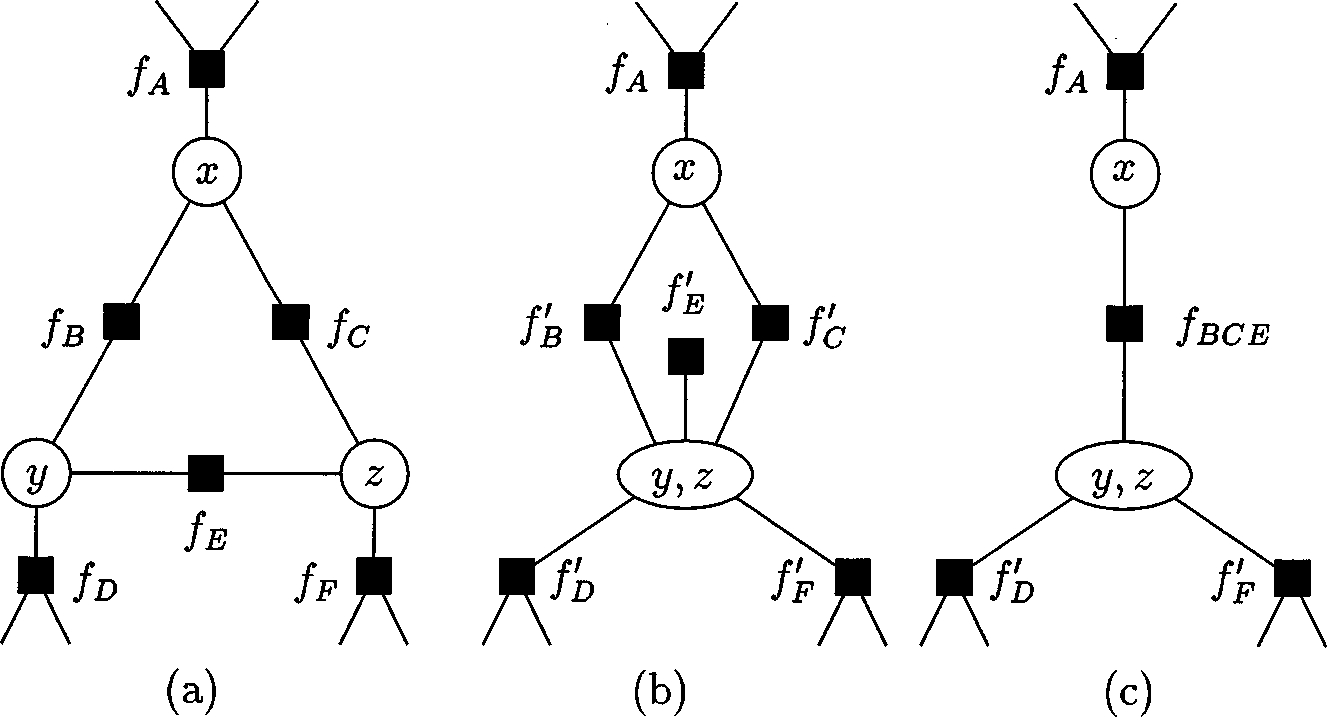
\includegraphics[width=0.8\textwidth]{fig/kschischang2001-clutering.png}
	\caption{Transformation: Clustering\cite{kschischang2001factor}}
\end{figure}	

Effect of clustering:
\begin{itemize}
	\item Cluster variable nodes: domain enlarged; no complexity increasing
	in local functions; increase complexity in sum-product algorithm
	(function evaluation). 
	\item Cluster function nodes: do not increase complexity of variables;
	increase complxity in sum-product algorithm
	(sizes of messages are increased). 
\end{itemize}

\begin{figure}[htb]
\centering
	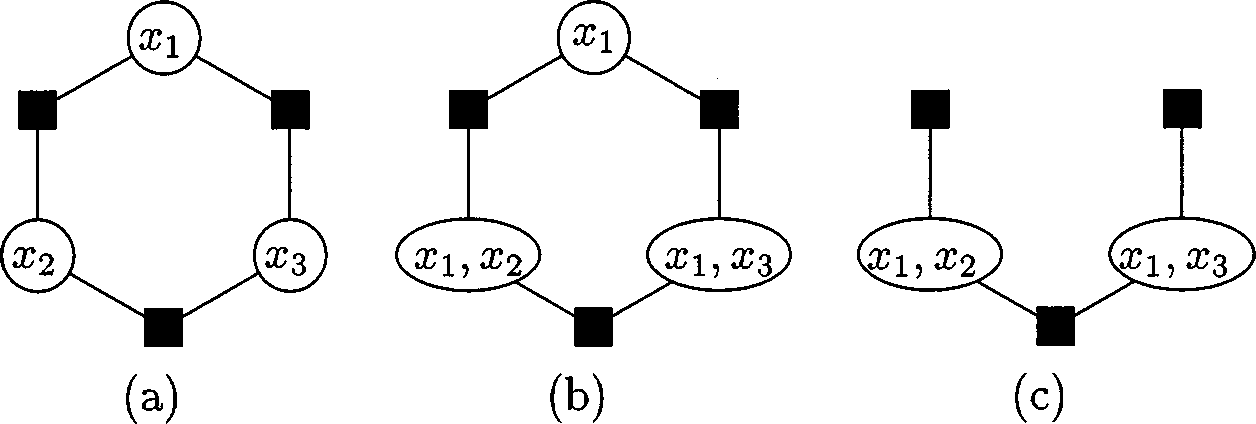
\includegraphics[width=0.8\textwidth]{fig/kschischang2001-streching.png}
	\caption{Transformation: Streching\cite{kschischang2001factor}}
\end{figure}

Effect of stretching:
\begin{itemize}
	\item Simply stretching variables adds positional variables to some local functions.
	Local function complexity is not changed. Variable alphabets are enlarged. 
	\item After stretching, redundant links or even redundant variables can be removed. 
	By systematic stretching, all cycles can be eliminated. 
\end{itemize}

\subsection{Parallelization}

The major advantage as we have already seen in previous examples
is, the locality of problems structure is captured by Factor Graph. 
Besides lowering the overall computation complexity, Factor Graph 
totally agrees with parallelization. 

For example, the famous MapReduce framework can be utilized 
to implement factor graph. Here we provide a short description 
of how to map factor graph to MapReduce framework. 
\begin{itemize}
	\item Both function nodes and variable nodes are unified 
	by one type of node, called unit. As we can see from the deduction 
	of FG, the operations performed on them are also the same. 
	\item Number of mappers is the same as number of reducers, 
	and the same as number of units.
	\item For every mapper, it calculates the multiplication of 
	all current messages together with the local function, and then 
	summarize it for every neighbouring nodes. After that, 
	it simply issue all new messages using the target node ID as the key. 
	\item For every reducer, it collects the list of messages targeted 
	for it and do nothing. Those collected messages can fit into 
	next round of map. 
	\item We run multiple round of MapReduce until a certain termination 
	criterion is reached. 
	\item To bootstrap the computation, the message list is initialized 
	as an identity message. 
\end{itemize}


\section{Selected Applications}

\subsection{Model System Dynamics}
This section follows the paper:\\
P.~Mirowski and Y.~LeCun.
\newblock Dynamic factor graphs for time series modeling.
\newblock {\em Machine Learning and Knowledge Discovery in Databases},
  v:128--143, 2009.
  
Declaration: figures in this section are borrowed from the orignal paper\cite{mirowski2009dynamic}. 
We omit further citation for simplicity.


\subsubsection{Quick Note of the Main Idea}

Problem settings:
\begin{itemize}
	\item System is composed of state variables and observation 
	variables. 
	\item Observation function maps state to observation. 
	\item Dynamic function governs state transitions. 
	\item Aim at modeling high dimensional underlying dynamic, 
	probably non-linear, but deterministc. 
\end{itemize}

\begin{figure}[htb]
\centering
	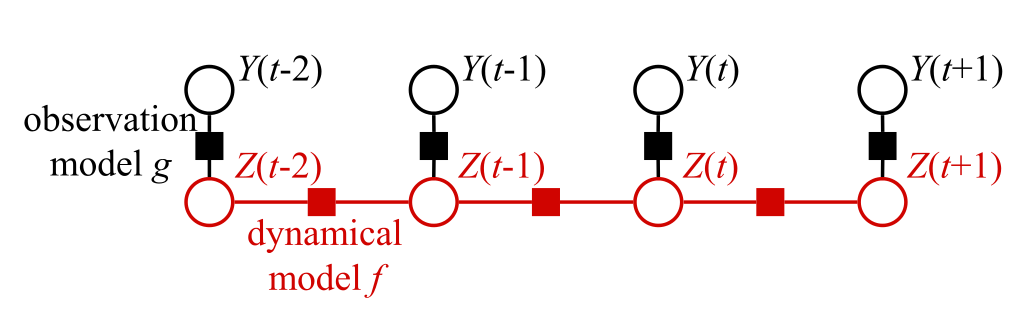
\includegraphics[width=0.8\textwidth]{fig/mirowski2009-HMM.png}
	\caption{Single State Dependency(HMM)}
\end{figure}	

When current state is only dependent on previous one state, it
is like an HMM model. 

\begin{figure}[htb]
\centering
	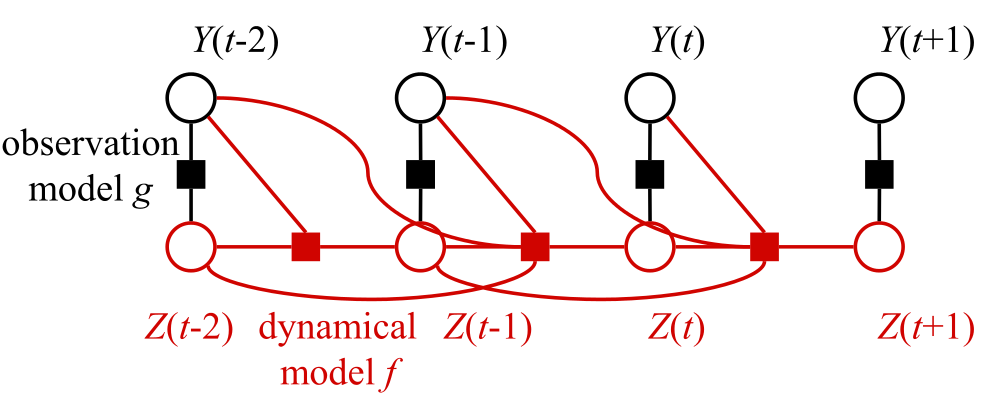
\includegraphics[width=0.8\textwidth]{fig/mirowski2009-framework.png}
	\caption{Multiple States and Observation Dependency}
\end{figure}

The state transition model can be more general that it may depend
on several previous states, or even observations. 

\begin{figure}[htb]
\centering
	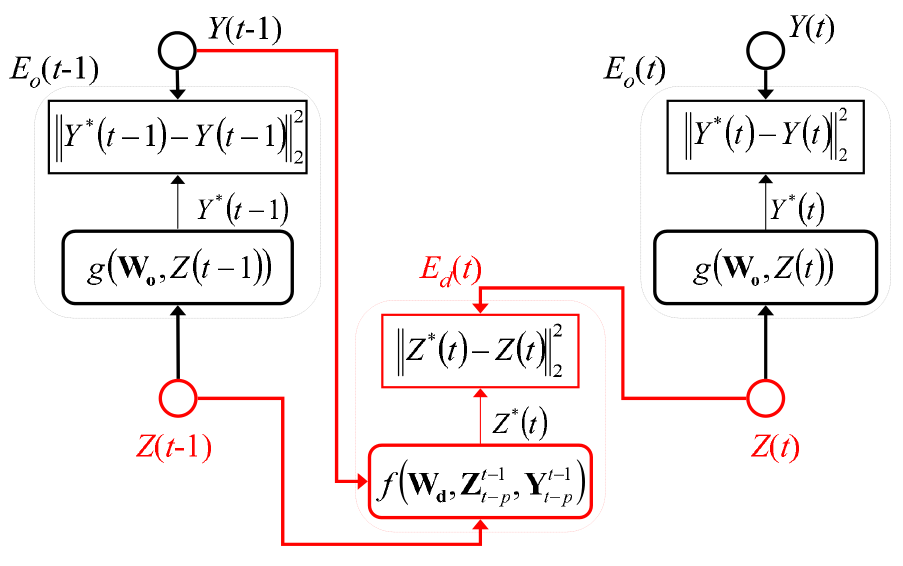
\includegraphics[width=0.8\textwidth]{fig/mirowski2009-detail.png}
	\caption{System Details}
\end{figure}

Formulation of paramterized FG:
\begin{eqnarray}
	L(\mathbf{W}, Y, Z) &=& E(\mathbf{W}, Y) + R_z(Z) + R(\mathbf{W}) \\
	\tilde{Z} &=& \argmax_{Z} L(\tilde{\mathbf{W}}, Y, Z) \label{eq:dfg-e}\\
	\tilde{\mathbf{W}} &=& \argmax_{\mathbf{W}} L(\mathbf{W}, Y, \tilde{Z})
	\label{eq:dfg-m}
\end{eqnarray}
Since the paper operates in the negative log domain, they want to minimize
$L$. The more likely some configuration is, the energy $E$ is lower. As is 
depicted in fig(), energy function is the square error. 

When parameters are fixed, eqn(\ref{eq:dfg-e}) acts as what ordinary 
factor graph does, namely, given all explicit function definitions, 
compute the marginalization problem. In ths application, paramters $\mathbf{W}$
is not determined. An usual way to tackle with this problem is 
by Expectation-Maximization schema (sometimes called Generalized Expectation 
Maximization algorithm). eqn(\ref{eq:dfg-e}) resembles the E-step, while 
eqn(\ref{eq:dfg-m}) resembles the M-step. 

\begin{figure}[htb]
\centering
	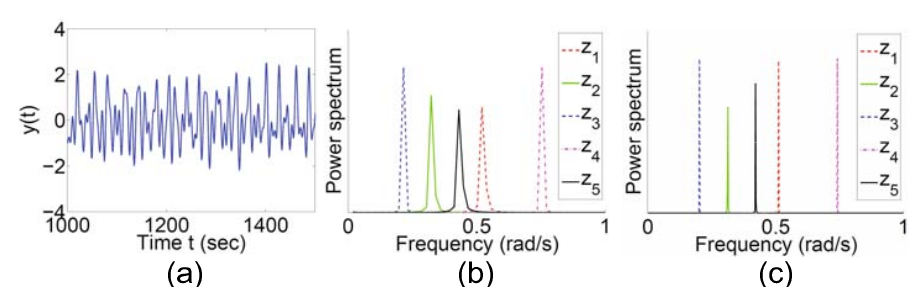
\includegraphics[width=0.8\textwidth]{fig/mirowski2009-sine.png}
	\caption{Training and Evaluation on Superimposed Sine Waves}
\end{figure}

To decouple 5 superimposed sine waves, the authors choose the architecture:
\begin{itemize}
	\item 5 dimensional state variable. 
	\item Dynamic function(f): 5 independent FIR filter of order 25. 
\end{itemize}

\begin{figure}[htb]
\centering
	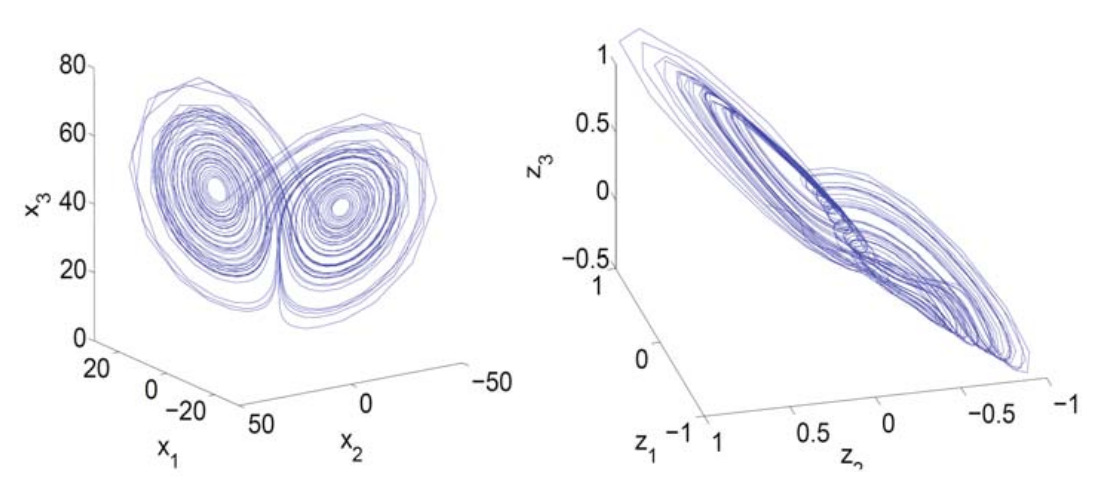
\includegraphics[width=0.8\textwidth]{fig/mirowski2009-Lorenz.png}
	\caption{Training and Evaluation on Lorenz Curve}
\end{figure}
To capture the observation of 1D variable whose underlying 
dynamic is 3D-Lorenz curve, the authors choose the architecture:
\begin{itemize}
	\item 3 dimensional state variable. 
	\item Dynamic function(f): 3 layered convelutional network. 
\end{itemize}

Besides the two evaluation mentioned above, the original paper
contains more. Interested readers can refer to \cite{mirowski2009dynamic} for 
more information. 

\subsubsection{Comments}

\begin{itemize}
	\item DFG(in this paper) is basically FG. 
	"dynamic" only address the application aspects, rather 
	than claiming an extension of FG. 
	\item The framework of FG is too general. 
	Designing observation function and state transition function, 
	choice of regularizer, setting coefficients are really tricky.
	There doesn't seem to be a rule of thumb. 
	\item The introduction of unknown parameters and regularizers
	make the formulation deviate from ordinary factor graph. 
	Before final marginalization, there is a training stage 
	to obtain opimal paramters. 
\end{itemize}

\subsection{Solving Marginalization Problem in Social Network}
This section follows the paper:\\
C.~Wang, J.~Tang, J.~Sun, and J.~Han.
\newblock Dynamic social influence analysis through time-dependent factor
  graphs.
\newblock {\em ASONAM}, v:p, 2011.

Declaration: figures in this section are borrowed from the orignal paper
\cite{wang2011-dynamic}. 
We omit further citation for simplicity. 

\subsubsection{Quick Note of the Main Idea}

Problem settings:
\begin{itemize}
	\item Graph $G^t=<V^t,E^t>$. $V$ corresponds to people in a certain 
	social network. $E$ corresponds activity relationships. There is 
	a real valued wegith function $w$ defined on $E$. 
	\item Graph $G^t$ captures time varying relationships. 
	\item Definition of $w$ is problem(application) specific. 
	\item Want to find the pairwise influence $\mu_{ij}$. Denote 
	the node to influence node $i$ by $y_i$, a random variable . 
	$\mu_{ij}$ is $P(y_i=j)$. 
\end{itemize}

\begin{figure}[htb]
\centering
	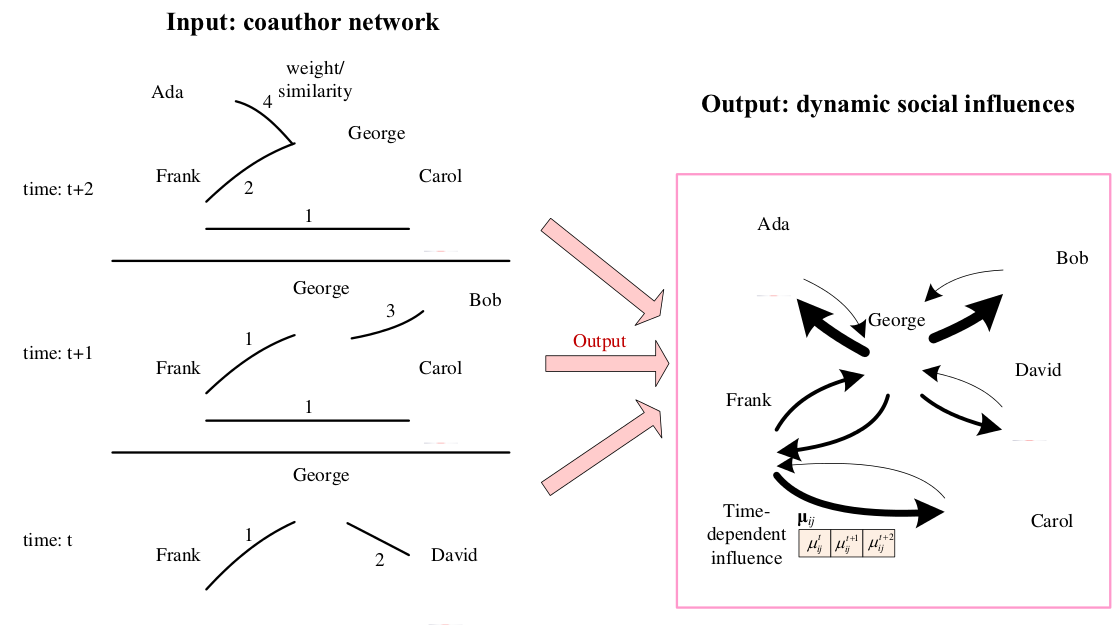
\includegraphics[width=0.8\textwidth]{fig/wang2011-problem.png}
	\caption{Problem Definition}
\end{figure}

When defined on the static version, one $\mu_{ij}$ is output for 
each $i,j$. When defined on the dynamic version, a vectore
$(\mu^{(t)}_{ij})$ is output. 

\begin{figure}[htb]
\centering
	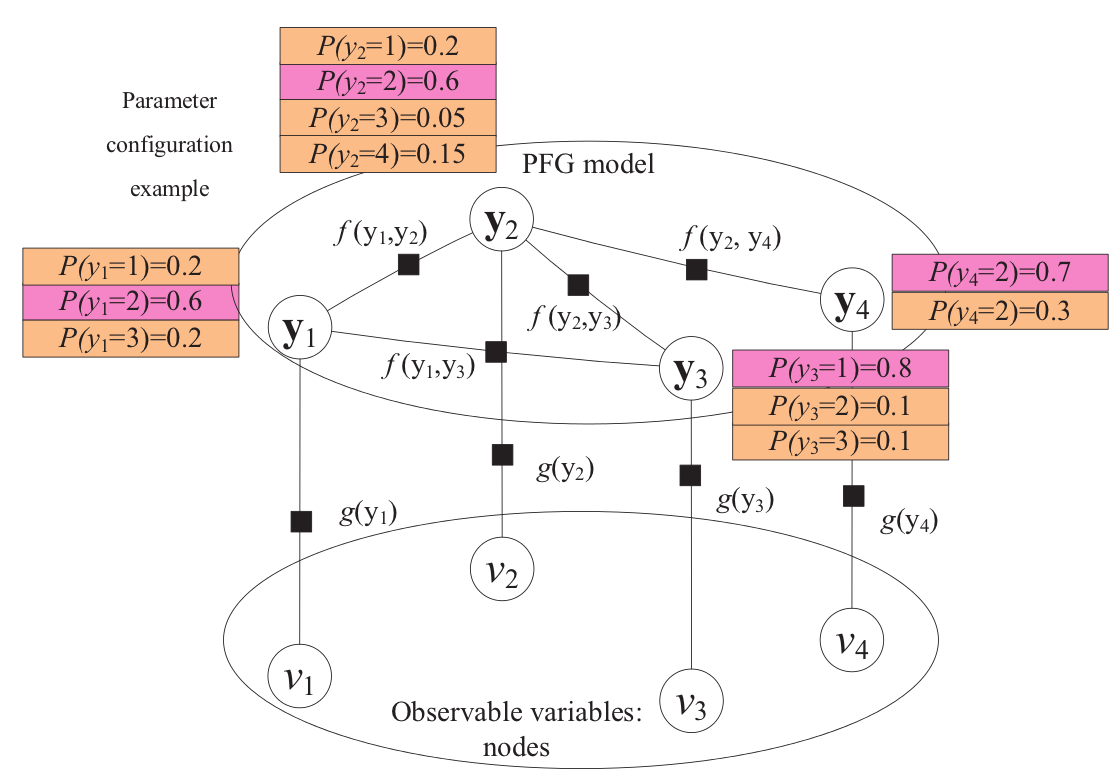
\includegraphics[width=0.8\textwidth]{fig/wang2011-FG-vis.png}
	\caption{Visualization of the Factor Graph}
\end{figure}

Two definitions to facilitate further description:
\begin{itemize}
	\item $NB(i)$: the neighbourhood of $i$. (More precisely, 
	$v_i$, this is defined on the original graph)
	\item $SC(i) = NB(i) \cup i$. 
\end{itemize} 

More precisely, $y_i$ should be linked to $v_j, \forall j \in NB(i)$
in the FG depicted in fig(). This can be justified through the definition
of node factor function. 

\begin{figure}[htb]
\centering
	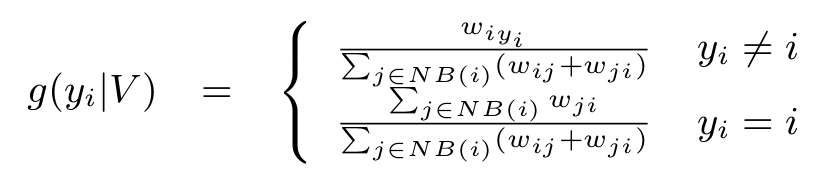
\includegraphics[width=0.8\textwidth]{fig/wang2011-nodefactor.png}
	\caption{Choice of Node Factor Function}
\end{figure}

\begin{figure}[htb]
\centering
	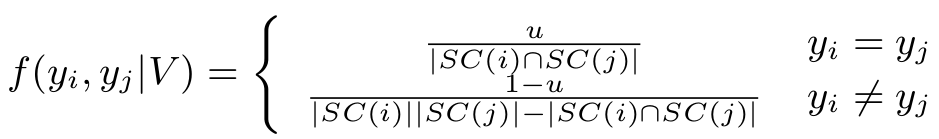
\includegraphics[width=0.8\textwidth]{fig/wang2011-edgefactor.png}
	\caption{Choice of Link Factor Function}
\end{figure}

The definition of node factor function and link factor function, together 
with the observation of $G$ removes complex links from $y_i$ to $V$. The 
resultant FG can be viewed as one single layer with $y_i$ vertices 
as variable nodes. Function nodes $g_i(y_i)$ are completely defined 
with the observation of $G$. 

Note that there is one parameter $u$ in the choice of 
link factor function. If not for this paramter, the FG in this paper
was able to marginalize each $y_i$ directly and give the influence 
using $\mu_{ij} = P(y_i=j)$. Again, the parameter estimation can be done
using EM schema. 

\begin{figure}[htb]
\centering
	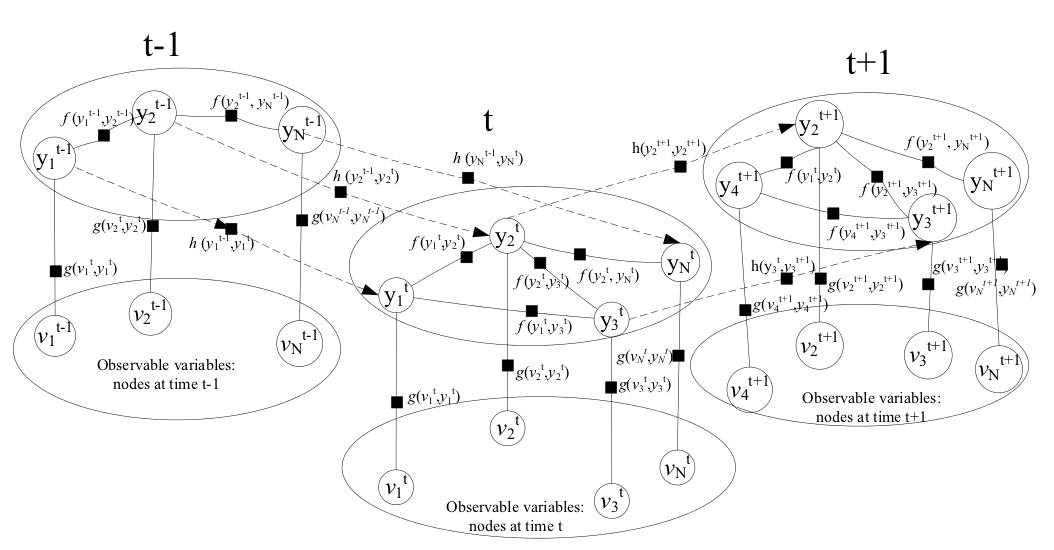
\includegraphics[width=0.8\textwidth]{fig/wang2011-FG-dynamic.png}
	\caption{Factor Graph with Time Dependency}
\end{figure}

In order to capture the time varying property of social influence, the 
authors augmented original static FG to be time-dependent FG. Bridging 
function nodes are added between two time consecutive sub graphs. For 
detailed discussion, please refer to original paper. 

Since the current section aims at modeling, details of algorithms are 
omitted. However, it's worth referring to the original paper for 
a specialized message passing algorithm named SIP(Social Influence 
Propagation) by the authors. That algorithm works more efficiently 
than general junction tree algorithms. 

\subsubsection{Comments}

\begin{itemize}
	\item Modeling an FG is rather easy. However, coming up with 
	right choice of functions and paramters are difficult. 
	\item In this paper, the authors used heuristics to generate 
	$w_{ij}$, which is a very important raw data. After the calculation 
	of $w_{ij}$, the FG and so does the marginalizations are fully defined. 
	\item The original itention(we've already shown that at the beginning
	of this article) of FG is to reduce complexity by utilizing graphical 
	structures. However, the compuation in practice is still a concern. 
	How to carefully design the algorithm to perform marginalization 
	under the message passing framework according to physical 
	meanings will be an interesting and chanllenging problem.   
\end{itemize}

\subsection{Short Summary on the Application of FG}

\begin{itemize}
	\item Framework and general algorithm is mature both in 
	theory and in practice. 
	\item Original FG can be used to solve marginalization problem 
	directly. At this point, FG can be think of as a problem solver
	rather than a model. For this flavour, please refer to Bishop's book
	\cite{bishop2006pattern}, Chapter 8. The author begins with 
	BN and MRF which model directed and undirected independencies. 
	In order to solve the inference problem, the author propose to 
	convert BN and MRF to FG. 
	\item According to different backgrounds, different authors 
	come up with different Paramterized Factor Graph. 
	Most of the works include two efforts: 
		\begin{itemize}
			\item Heuristics to determine paramters. 
			\item Iterative methods to determine paramters. 
			(EM schema)
		\end{itemize}			
	Solving marginalization in FG is one sub problem then. Before
	giving the final marginalized answer, there is a training stage. 
	\item Specific message passing algorithms are worth investigating. 
	As is in \cite{wang2011-dynamic}, the authors propose SIP, specialized 
	for their problem. The resulting algorithm is more tractable than 
	general solvers. 
\end{itemize}

\section{Other Taste of Modeling}

\subsection{Coding}

Besides modeling probability problems, people also use FG to 
model certain codes. 

Consider a parity checking matrix given by $H$:
\begin{equation}
	H = \left[
	\begin{matrix}
		1 & 1 & 0 & 0 & 1 & 0 \\
0 & 1 & 1 & 0 & 0 & 1 \\
1 & 0 & 1 & 1 & 0 & 0 \\
	\end{matrix}
	\right]
\end{equation}

In the corresponding factor graph, each factor node corresponds
to one row and each variable node corresponds to one column. The 
type of the functions are indicators testing the predicate:
$[x_{i_1} \oplus x_{i_2} \oplus x_{i_1} = 0]$. Note that 
the logic "$\cap$" operator can be regarded as "product". 
This kind of modeling is called behavioural modeling in 
\cite{kschischang2001factor}. 

\begin{figure}[htb]
\centering
	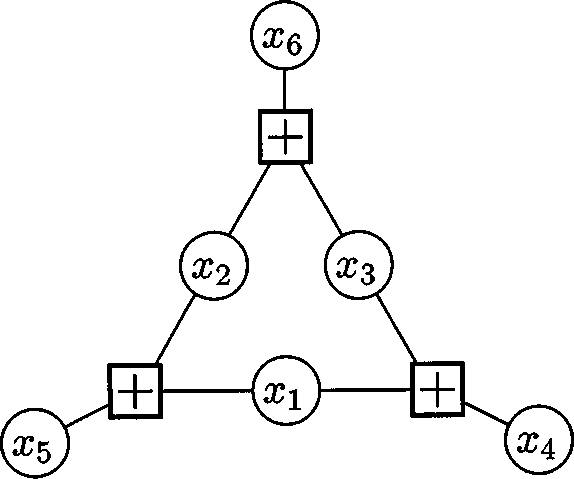
\includegraphics[width=0.4\textwidth]{fig/kschischang2001-parity}
	\caption{A Parity Code Modeled by FG\cite{kschischang2001factor}}
\end{figure}


\subsection{Subgame Perfect Equilibrium}

Interestingly, to search the subgame perfect equilibrium of 
an extensive game, we can use factor graph. For detailed 
course materials on extensive game, interested readers can 
refer to \cite{osborne1994course}. 

We know that to find the Nash Equilibrium of a game, 
one can enumerate the set of strategy profiles, and 
check for every player whether he can gain by deviation. 
This method is time-consuming, since it is no more than 
the definition of an equilibrium. However, subgame perfect 
equilibrium can be found much more efficiently with the help 
of One Deviation Property Lemma\cite{osborne1994course}. 
The lemma says, for every subgame of original game, we 
only need to check whether the first move is optimal or not. 
More intuitively, we can do backward deduction on the tree
from leaves to root. 

Note that in our introduction to FG, the example that we marginalize
for a tree structure with a designated root fits this compuation very 
well. 


\section{Related Models/Algorithms}

Models:
\begin{itemize}
	\item Bayesian Network. Directed Graphical Model. 
	\item Markov Random Field. Undirected Graphical Model.
	\item Chain Graph. Directed + Undirected.  
	\item Factor Graph. 
\end{itemize}

\begin{figure}[htb]
\centering
	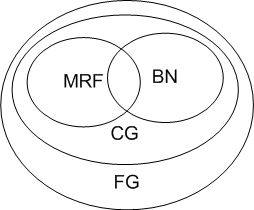
\includegraphics[width=0.3\textwidth]{illustration/graphical-venn.png}
	\caption{Venn Graph of Several Graphical Models}
\end{figure}

Justification of modeling ability:
\begin{itemize}
	\item BN $\rightarrow$ MRF. The moralization process hides certain stucture 
	previously available in BN. 
	\item MRF. An example of square located 4 nodes. If two diagonal variables 
	are observed, the other two variables become independent. BN can not express 
	such information. 
	\item CG. Since both directed and undirected, it forms the superset of 
	the union of BN and	MRF.
	\item FG. Converting CG to FG reveals more details, namely, how the joint 
	distribution is factorized(usually, one explicit normalization function 
	exhibits). BTW, FG can model not only probabilistic problems, but also 
	other problems like system dynamics and coding. It is super general in the
	sense.
\end{itemize}


Algorithms:
\begin{itemize}
	\item Junction tree. 
	\item Bayesian ball. 
	\item (Loopy)Belief propagation. 
	\item Sum-product. 
\end{itemize}

\section{Discussions}

Since the development of factor graph is boosted in the past decade, 
different authors come up with different description of similar problems. 
Not to distinguish right from wrong, I just regard those stuffs out there
as inconsistent. My opinion on some parts of past literature:
\begin{itemize}
	\item In Bishop's book\cite{bishop2006pattern}, chapter 8.4.5, P411. 
	The example is not good. Actually, when talking about that probability 
	maximization problem, we should know "product" corresponds to product operator, 
	and "sum" corresponds to max operator. In this case, the maginalization 
	operation for a single varialbe is indeed the maximization for each 
	instancde of that variable. Using local marginalized function(max), we 
	can certainly get the global probability maximization point considering
	all variables. 
	\item As for Dynamic Factor Graph, the author of this paper do not advocate 
	the abuse of this term like an extension of factor graph. FG itself is able 
	to model system dynamics, as we've already seen in those examples above. 
	Other authors may use the term DFG
\cite{wang2011-dynamic}
\cite{mirowski2009dynamic}
	, but their DFG is application specific. 
	Those graphs are essentially FG. Not until we examine the physical meaning of 
	some factor nodes do we realize their "dynamic" property. 
\end{itemize}

\section*{Acknowledgements}

\input{../reference/gen_bib.bbl}

\end{document}